% IEEE conference format. Build: pdflatex paper; bibtex paper; pdflatex paper; pdflatex paper
\documentclass[conference]{IEEEtran}
\usepackage{cite}
\usepackage{amsmath}
\usepackage{graphicx}
\usepackage{booktabs}
\usepackage{url}
\graphicspath{{../results/}}

\begin{document}

\title{Fine-Tuned Vision Transformer for 38-Class Plant Leaf Disease Classification with Attention-Rollout Explanations and Efficiency Benchmarking}

\author{
\IEEEauthorblockN{Tushar Singh\textsuperscript{*}}
\IEEEauthorblockA{\textit{School of Computer Science and Engineering}\\
\textit{IILM University}\\
Greater Noida, India\\
tushar.singh.cs28@iilm.edu}
\and
\IEEEauthorblockN{Anurodh Singh}
\IEEEauthorblockA{\textit{School of Computer Science and Engineering}\\
\textit{IILM University}\\
Greater Noida, India\\
anurodh.singh.cs28@iilm.edu}
\and
\IEEEauthorblockN{Vansh Thakur}
\IEEEauthorblockA{\textit{School of Computer Science and Engineering}\\
\textit{IILM University}\\
Greater Noida, India\\
vansh.thakur.cs28@iilm.edu}
\and
\IEEEauthorblockN{Sahil Sharma}
\IEEEauthorblockA{\textit{School of Computer Science and Engineering}\\
\textit{IILM University}\\
Greater Noida, India\\
sahil.sharma.cs28@iilm.edu}
\thanks{\textsuperscript{*}Corresponding author.}}

\maketitle

\begin{abstract}
Plant-leaf classifiers trained on PlantVillage routinely report accuracy above 99\%, but the dataset contains several photographs of the same leaf, so reported accuracy can overstate performance on unseen leaves, and large transformers are rarely compared with lightweight CNNs on deployment cost. We fine-tune ViT-B/16 and MobileNetV2 on the 38 PlantVillage classes using a near-duplicate-aware split that keeps images of the same leaf in one partition. Over three training seeds on 8,155 held-out images, ViT-B/16 reaches 99.87\% accuracy (SD 0.04) and MobileNetV2 99.76\% (SD 0.02). ViT is ahead on every seed by 0.06 to 0.15 points, but the paired McNemar test is significant on only one of the three seeds, so the advantage is small. ViT-B/16 needs 85.8\,M parameters against 2.27\,M and 223\,ms against 22.8\,ms CPU latency per image. A deletion test of attention-rollout maps shows a modest faithful ordering of patches, but the maps do not concentrate on the leaf more than its area share. Remaining errors are mostly between maize Northern Leaf Blight and Gray Leaf Spot. A plain random split gave similar accuracy, so we found no measurable inflation from near-duplicate leakage on this dataset. Results come from PlantVillage only, so they do not show how the models behave on field images.
\end{abstract}

\begin{IEEEkeywords}
plant disease classification, vision transformer, MobileNetV2, attention rollout, PlantVillage, efficiency benchmarking
\end{IEEEkeywords}

\section{Introduction}
Automated recognition of plant disease from leaf photographs has been studied since deep networks were first applied to PlantVillage \cite{mohanty2016,ferentinos2018}, and reviews have long warned that images taken under controlled conditions limit what such systems achieve in the field \cite{barbedo2016}.

\textbf{Problem.} Classifiers trained on PlantVillage routinely report accuracy above 99\%, yet the dataset contains several photographs of the same leaf and background cues that correlate with the label \cite{noyan2022bias}. Reported accuracy can therefore overstate how well a model works on unseen leaves, and large transformer models are rarely compared with lightweight CNNs on deployment cost.

\textbf{Research question.} On a split that keeps near-duplicate photographs together, does a fine-tuned Vision Transformer (ViT) \cite{dosovitskiy2021vit} outperform MobileNetV2 \cite{sandler2018mobilenetv2} on 38-class classification, and does any accuracy gain justify its extra parameters and inference latency? A secondary question is whether attention-rollout maps \cite{abnar2020rollout} highlight the diseased leaf rather than the background.

\textbf{Contributions.}
\begin{enumerate}
\item We fine-tune ViT-B/16 on 38 PlantVillage classes with a near-duplicate-aware split and report 99.89\% accuracy and macro F1 of 0.9976 on 8,155 held-out images for seed 42 (95\% CI 99.82--99.95\%; three-seed mean 99.87\%).
\item We compare it with MobileNetV2 under the same split and training budget. Over three seeds ViT is ahead by 0.11 points on average (0.06 to 0.15), but the McNemar test is significant on only one seed ($p=0.078$, $0.017$, $0.42$), so the advantage is small, while ViT costs 85.8\,M versus 2.27\,M parameters, 343\,MB versus 9.3\,MB, and 223\,ms versus 22.8\,ms CPU latency per image.
\item We compute attention-rollout maps and test them with a deletion check on 400 correctly classified images. Removing the top-ranked 25\% of patches lowers the true-class probability about twice as much as removing random patches (0.029 versus 0.015), but the maps do not concentrate on the leaf more than its area share, so we make no localisation claim.
\item We measure near-duplicate leakage: under a plain random split 6.9\% of test images have a same-group image in training (none under ours), yet random-split accuracy was not higher (99.85\% against 99.89\% for ViT-B/16, one seed, different test sets), and the weakest class F1 is 0.967 (maize Cercospora/Gray Leaf Spot, whose errors are mostly Northern Leaf Blight images predicted as Gray Leaf Spot), with all 38 classes for both models in the appendix.
\end{enumerate}

\section{Related Work}
PlantDoc was built to test models on field images \cite{singh2020plantdoc}, and an audit of PlantVillage showed that a model given only 8 background pixels reached 49\% accuracy against 2.6\% for chance \cite{noyan2022bias}. Vision transformers \cite{dosovitskiy2021vit,touvron2021deit} have since been applied to plant disease alone \cite{borhani2022}, combined with CNNs \cite{thakur2023plantxvit}, as lightweight hybrids \cite{tonmoy2025mobileplantvit}, with a mixture of experts for field data \cite{salman2025moe}, and compared with CNNs and CLIP \cite{radford2021clip} under domain shift \cite{benabbas2025rethinking}; surveys are given in \cite{mehdipour2025vitagri,banerjee2025eval}. Explanation methods for transformers include attention rollout \cite{abnar2020rollout} and gradient-based relevance \cite{chefer2021beyond}, Grad-CAM is the usual choice for CNNs \cite{selvaraju2017gradcam}, and attention weights alone are not always faithful explanations \cite{jain2019attention}.

Table~\ref{tab:published} lists published PlantVillage and PlantDoc results next to ours. Published PlantVillage results are very high: 99.9\% for an encoder--decoder transformer \cite{feng2024encdec} and above 99.3\% for a hierarchical ViT on a tomato-leaf subset of PlantVillage, as reported in the survey \cite{banerjee2025eval}. Accuracy falls on field images: a ViT with a mixture of experts reaches 68\% when trained on PlantVillage and tested on PlantDoc \cite{salman2025moe}. Our 99.89\% on PlantVillage is in the same range as the published figures. Because protocols differ (split, augmentation, pretraining), direct ranking is not meaningful, and we did not test cross-dataset transfer. We add a comparison of a fine-tuned ViT-B/16 and MobileNetV2 under a near-duplicate-aware split, with deployment cost and a deletion test of the rollout maps.

\begin{table}[t]
\caption{Published PlantVillage / PlantDoc results (protocols differ; not directly comparable). ``Ours'' rows are three-seed means on the near-duplicate-aware split.}
\label{tab:published}
\centering
\footnotesize
\begin{tabular}{@{}p{1.5cm}p{2.0cm}p{2.5cm}r@{}}
\toprule
Work & Model & Dataset / split & Accuracy \\
\midrule
\mbox{\cite{feng2024encdec}} & Encoder--decoder transformer & PlantVillage, authors' protocol & 99.9\% \\
\mbox{\cite{banerjee2025eval}} & Hierarchical ViT (as reported in the survey) & PlantVillage tomato-leaf subset, survey's evaluation & $>$99.3\% \\
\mbox{\cite{salman2025moe}} & ViT with mixture of experts & PlantVillage $\rightarrow$ PlantDoc & 68\% \\
Ours & ViT-B/16 & PlantVillage, grouped split & 99.87\% \\
Ours & MobileNetV2 & PlantVillage, grouped split & 99.76\% \\
\bottomrule
\end{tabular}
\end{table}

\section{Data and Method}
\subsection{Dataset and split}
We use the PlantVillage color images (54,305 images, 38 classes) from the public repository of Mohanty \emph{et al.} \cite{mohanty2016}, git commit \texttt{7f7ecc7}, original data from \cite{hughes2015plantvillage}. We cloned the repository on 26 November 2026; it has no licence file, but the front matter of its \texttt{README\_HF.md} declares CC BY-SA 3.0. PlantVillage photographs the same leaf several times. We hash every image with a rotation- and flip-invariant difference hash, link images of the same class whose 64-bit hashes differ by at most 6 bits, and split by connected component into train (37,860), validation (8,290) and test (8,155) images, stratified by class. Of the 54,305 images, 4,425 fall in groups of more than one image, and the largest group has 332 images. Under a plain random split 6.9\% of test images have a same-group image in training; under our split none do. The grouping is approximate, so we call the split near-duplicate-aware, not leaf-level. The split list is released with the code.

\subsection{Models and training}
We fine-tune ViT-B/16 (\texttt{vit\_\allowbreak{}base\_\allowbreak{}patch16\_\allowbreak{}224.augreg\_\allowbreak{}in21k\_\allowbreak{}ft\_\allowbreak{}in1k}, ImageNet-21k pretraining followed by ImageNet-1k fine-tuning \cite{steiner2022augreg}) and MobileNetV2 (\texttt{mobilenetv2\_\allowbreak{}100.ra\_\allowbreak{}in1k}) from the timm library, replacing the head with 38 outputs. Both use AdamW (weight decay 0.05), a one-cycle schedule, batch size 32, mixed precision and 3 epochs, with learning rate $3\times10^{-5}$ for ViT and $10^{-3}$ for MobileNetV2. Training augmentation is random resized crop (scale 0.6--1.0), horizontal and vertical flips and colour jitter, at $224\times224$. We keep the epoch with the best validation accuracy and evaluate it once on the test set. We train each model with three seeds (42, 43, 44); the split is fixed. We also train both models once (seed 42) on a plain stratified random split to check for leakage effects.

\subsection{Evaluation}
We report accuracy, macro and weighted precision, recall and F1 with 95\% bootstrap confidence intervals, per-class results, and a McNemar test on paired test predictions. Macro F1 was also computed by hand as the mean of the 38 per-class values and matches the library value. Latency, size and operation counts use the fine-tuned architectures at batch size 1 on 4 CPU threads and on a laptop GPU (RTX 4050), plus fp16 throughput at batch size 64.

\subsection{Attention rollout checks}
We compute attention rollout \cite{abnar2020rollout} for 400 correctly classified test images. First, we compare the share of rollout attention inside an approximate leaf mask with the share of the image the mask covers. Second, in a deletion test we zero the top-ranked 10\% or 25\% of patches by rollout, the same number of random patches, or the lowest-ranked patches, and record the drop in true-class probability. A faithful ranking should drop the probability more than random.

\section{Results}
\subsection{Classification}
Table~\ref{tab:seeds} gives the three seeds, and Table~\ref{tab:main} the full seed-42 results. Across seeds ViT-B/16 reaches 99.87\% test accuracy (SD 0.04) and MobileNetV2 99.76\% (SD 0.02), with macro F1 0.9979 and 0.9957. ViT is ahead on every seed, by 0.11, 0.15 and 0.06 points. On the images where the two models disagree, ViT is right and MobileNetV2 wrong on 15, 17 and 15 images, and the reverse on 6, 5 and 10; the McNemar test gives $p=0.078$, $0.017$ and $0.42$. The seeds share one test set, so these tests are not independent. We read this as a small advantage for ViT of about 0.1 points that a single run cannot establish, and we do not claim a larger one.

\begin{table}[t]
\caption{Test accuracy of the three seeds on the near-duplicate-aware split (same test set), and one run on a plain random split (a different test set of 8,146 images, so not paired with the rows above).}
\label{tab:seeds}
\centering
\small
\begin{tabular}{lrr}
\toprule
 & ViT-B/16 & MobileNetV2 \\
\midrule
Grouped, seed 42 & 0.9989 & 0.9978 \\
Grouped, seed 43 & 0.9989 & 0.9974 \\
Grouped, seed 44 & 0.9983 & 0.9977 \\
Grouped, mean (SD) & 0.9987 (0.0004) & 0.9976 (0.0002) \\
\midrule
Random split, seed 42 & 0.9985 & 0.9958 \\
\bottomrule
\end{tabular}
\end{table}

The random split uses a different test set (8,146 images), so its accuracy is not directly paired with the grouped runs. It gave 99.85\% for ViT and 99.58\% for MobileNetV2, which is not higher than on the grouped split, so we found no measurable inflation from near-duplicate leakage here.

\begin{table}[t]
\caption{Test results on the near-duplicate-aware split (8,155 images, seed 42) and deployment cost.}
\label{tab:main}
\centering
\small
\resizebox{\columnwidth}{!}{%
\begin{tabular}{lrr}
\toprule
 & ViT-B/16 & MobileNetV2 \\
\midrule
Accuracy & 0.9989 & 0.9978 \\
Accuracy 95\% CI & 0.9982--0.9995 & 0.9967--0.9988 \\
Macro precision & 0.9980 & 0.9965 \\
Macro recall & 0.9974 & 0.9946 \\
Macro F1 & 0.9976 & 0.9955 \\
Weighted F1 & 0.9989 & 0.9978 \\
\midrule
Parameters (M) & 85.8 & 2.27 \\
Size, fp32 (MB) & 343 & 9.3 \\
GMACs & 16.9 & 0.31 \\
CPU latency, batch 1 (ms) & 223 & 22.8 \\
GPU latency, batch 1, fp32 (ms) & 12.8 & 6.8 \\
GPU throughput, batch 64, fp16 (img/s) & 382 & 1924 \\
\bottomrule
\end{tabular}}
\end{table}

\subsection{Weakest classes}
For ViT-B/16 the lowest F1 values are maize Cercospora/Gray Leaf Spot (0.967), potato healthy (0.976; 21 test images), maize Northern Leaf Blight (0.983), tomato spider mites (0.994), tomato Target Spot (0.995) and blueberry healthy (0.998). The most frequent error is maize Northern Leaf Blight predicted as Gray Leaf Spot (4 images), followed by tomato spider mites predicted as Target Spot (2). MobileNetV2 shows the same maize confusion (4 and 3 images). All 38 classes are in the appendix (Tables~\ref{tab:perclass_vit} and~\ref{tab:perclass_mnv2}).

\subsection{Cost}
ViT-B/16 has about 38 times the parameters, 54 times the operations and about 10 times the CPU latency of MobileNetV2, and its batch-64 GPU throughput is about five times lower. GPU latency at batch size 1 differs by less (12.8\,ms versus 6.8\,ms in fp32). Timings were taken on a laptop GPU and are noisy; for example MobileNetV2 was slower in fp16 than in fp32 at batch size 1, so we quote fp32 and CPU figures.

\subsection{Attention rollout}
Across the 400 images, a mean of 0.877 of the rollout attention falls inside the leaf mask, which covers a mean 0.885 of the image (median ratio 0.999; ratio above 1 on 41\% of images). Rollout therefore shows no preference for the leaf over the background, and because PlantVillage leaves fill most of the frame, this check is weak. In the deletion test, removing the top 25\% of patches lowers the true-class probability by 0.029, against 0.015 for random patches and 0.009 for the lowest-ranked patches; at 10\% the values are 0.0041, 0.0038 and 0.0016. The ordering is consistent but the effects are small, because the classifier is already very confident on these images. Fig.~\ref{fig:rollout} shows examples.

\begin{figure}[t]
\centering
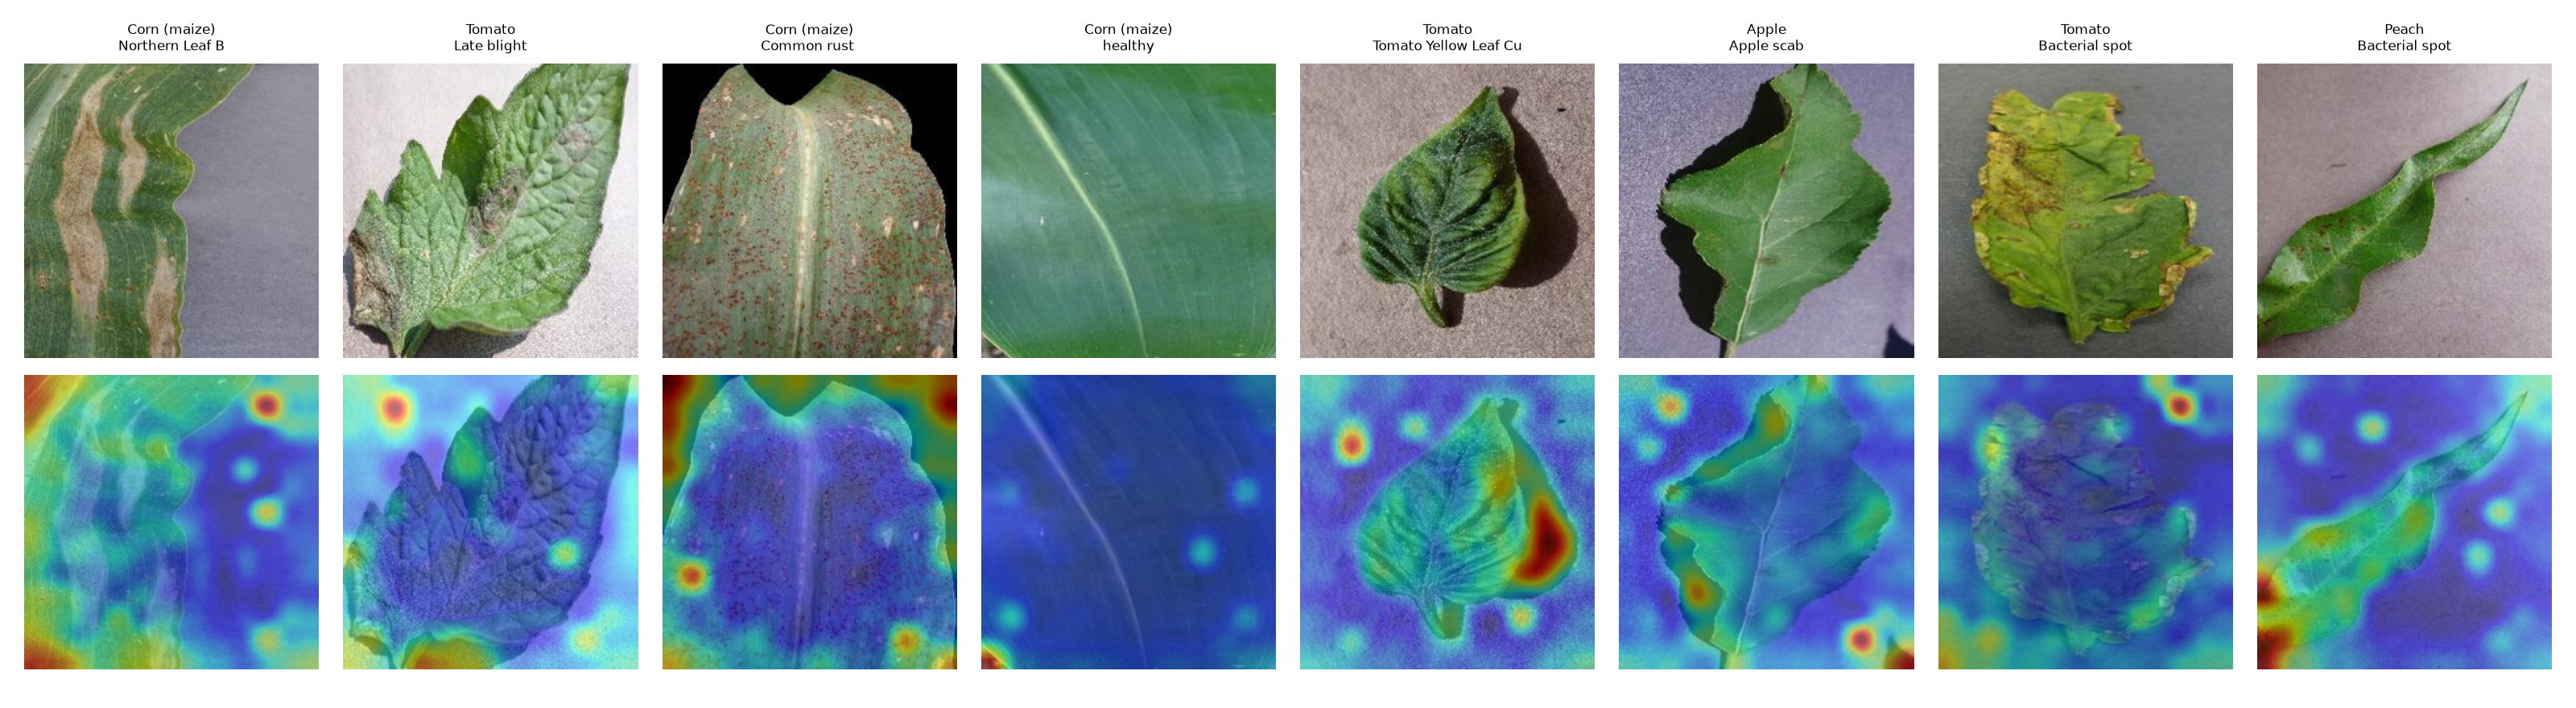
\includegraphics[width=\columnwidth]{fig_rollout.png}
\caption{Attention-rollout examples from the fine-tuned ViT-B/16 on correctly classified test images.}
\label{fig:rollout}
\end{figure}

\section{Discussion}
Both models are near ceiling on this split, so PlantVillage barely separates them: ViT is ahead by about 0.1 points across three seeds, a gap that is consistent in sign but small, and a ViT run costs far more. A CNN builds global context only through depth, whereas self-attention relates all patches from the first layer \cite{dosovitskiy2021vit}, but we did not test whether this matters for symptoms spread across the leaf, and we make no claim that ViTs capture dispersed symptoms better. For deployment on constrained devices, the evidence here favours MobileNetV2: it is within 0.11 points of ViT with under 3\% of the parameters.

The near-duplicate-aware split removes the same-leaf leakage that a random split has (6.9\% of test images). Training on the random split did not give higher accuracy than the grouped split (99.85\% and 99.58\% against 99.89\% and 99.78\%), although the test sets differ and we ran one seed, so we can only say that any inflation was too small to see. The accuracy we report is still on PlantVillage images with uniform backgrounds, and published results show large drops on field images \cite{salman2025moe,singh2020plantdoc}.

\section{Limitations}
(1) Three seeds and 3 epochs per model; the seeds share one split and test set, and the random-split comparison is a single run. (2) Hash-based grouping removes near-duplicates but does not guarantee that no leaf is shared across splits. (3) PlantVillage only; no cross-dataset test such as PlantDoc. (4) The leaf mask used in the rollout check is approximate, and the deletion test measures faithfulness to the model, not agreement with expert-marked lesions. (5) Latency was measured on one laptop GPU and one CPU configuration. (6) We did not compare explanations with Grad-CAM on MobileNetV2.

\section{Conclusion}
On a near-duplicate-aware PlantVillage split, fine-tuned ViT-B/16 and MobileNetV2 both exceed 99.7\% test accuracy over three seeds, with ViT-B/16 about 0.1 points ahead, significant on one seed of three, while it costs far more in parameters and latency. Rollout ranks patches in a modestly faithful way but does not localise the leaf. Future work should test cross-dataset transfer to field images, train for longer, and compare explanations across architectures.

\section*{Data and Code Availability}
Code, the split list (image path and train/validation/test assignment), training histories and result files are available at \url{https://github.com/tusharsingh-1801/91-CHM} (directory \texttt{docs/vit-paper}). The code is under the MIT licence, and the split list and result files are under CC BY-SA 3.0. The trained ViT-B/16 and MobileNetV2 weights (seed 42, near-duplicate-aware split) are released for research use as GitHub release \texttt{vit-paper-v1.0} of the same repository, with SHA-256 checksums in \texttt{release/README.md}; a snapshot of the repository at that release is archived on Zenodo (DOI \texttt{10.5281/zenodo.24590449}), which does not contain the weight files. They were trained on PlantVillage, so users must check the dataset terms (CC BY-SA 3.0 as declared upstream) before reuse. PlantVillage images are not redistributed; the source and commit are given above, and the source repository has no licence file but declares CC BY-SA 3.0 in its \texttt{README\_HF.md}, so users should check the terms of the copy they download.

\bibliographystyle{IEEEtran}
\bibliography{../references}

\appendices
\section{Per-class results for ViT-B/16}
\begin{table}[h]
\caption{Per-class precision, recall, F1 and support for ViT-B/16 on the test set.}
\centering
\tiny
\resizebox{\columnwidth}{!}{\begin{tabular}{lrrrr}
\toprule
class & precision & recall & f1 & support \\
\midrule
Apple\_\_\_Apple\_scab & 1.0000 & 1.0000 & 1.0000 & 93 \\
Apple\_\_\_Black\_rot & 1.0000 & 1.0000 & 1.0000 & 93 \\
Apple\_\_\_Cedar\_apple\_rust & 1.0000 & 1.0000 & 1.0000 & 40 \\
Apple\_\_\_healthy & 1.0000 & 1.0000 & 1.0000 & 247 \\
Blueberry\_\_\_healthy & 0.9956 & 1.0000 & 0.9978 & 225 \\
Cherry\_(including\_sour)\_\_\_Powdery\_mildew & 1.0000 & 1.0000 & 1.0000 & 158 \\
Cherry\_(including\_sour)\_\_\_healthy & 1.0000 & 1.0000 & 1.0000 & 128 \\
Corn\_(maize)\_\_\_Cercospora\_leaf\_spot Gray\_leaf\_spot & 0.9487 & 0.9867 & 0.9673 & 75 \\
Corn\_(maize)\_\_\_Common\_rust\_ & 1.0000 & 1.0000 & 1.0000 & 179 \\
Corn\_(maize)\_\_\_Northern\_Leaf\_Blight & 0.9931 & 0.9728 & 0.9828 & 147 \\
Corn\_(maize)\_\_\_healthy & 1.0000 & 1.0000 & 1.0000 & 174 \\
Grape\_\_\_Black\_rot & 1.0000 & 1.0000 & 1.0000 & 177 \\
Grape\_\_\_Esca\_(Black\_Measles) & 1.0000 & 1.0000 & 1.0000 & 207 \\
Grape\_\_\_Leaf\_blight\_(Isariopsis\_Leaf\_Spot) & 1.0000 & 1.0000 & 1.0000 & 161 \\
Grape\_\_\_healthy & 1.0000 & 1.0000 & 1.0000 & 63 \\
Orange\_\_\_Haunglongbing\_(Citrus\_greening) & 1.0000 & 1.0000 & 1.0000 & 879 \\
Peach\_\_\_Bacterial\_spot & 1.0000 & 1.0000 & 1.0000 & 317 \\
Peach\_\_\_healthy & 1.0000 & 1.0000 & 1.0000 & 54 \\
Pepper,\_bell\_\_\_Bacterial\_spot & 1.0000 & 1.0000 & 1.0000 & 149 \\
Pepper,\_bell\_\_\_healthy & 1.0000 & 1.0000 & 1.0000 & 221 \\
Potato\_\_\_Early\_blight & 1.0000 & 1.0000 & 1.0000 & 150 \\
Potato\_\_\_Late\_blight & 1.0000 & 1.0000 & 1.0000 & 150 \\
Potato\_\_\_healthy & 1.0000 & 0.9524 & 0.9756 & 21 \\
Raspberry\_\_\_healthy & 1.0000 & 1.0000 & 1.0000 & 55 \\
Soybean\_\_\_healthy & 1.0000 & 1.0000 & 1.0000 & 763 \\
Squash\_\_\_Powdery\_mildew & 1.0000 & 1.0000 & 1.0000 & 275 \\
Strawberry\_\_\_Leaf\_scorch & 1.0000 & 1.0000 & 1.0000 & 167 \\
Strawberry\_\_\_healthy & 1.0000 & 1.0000 & 1.0000 & 66 \\
Tomato\_\_\_Bacterial\_spot & 1.0000 & 1.0000 & 1.0000 & 318 \\
Tomato\_\_\_Early\_blight & 1.0000 & 1.0000 & 1.0000 & 150 \\
Tomato\_\_\_Late\_blight & 1.0000 & 1.0000 & 1.0000 & 287 \\
Tomato\_\_\_Leaf\_Mold & 1.0000 & 1.0000 & 1.0000 & 142 \\
Tomato\_\_\_Septoria\_leaf\_spot & 1.0000 & 1.0000 & 1.0000 & 266 \\
Tomato\_\_\_Spider\_mites Two-spotted\_spider\_mite & 0.9960 & 0.9920 & 0.9940 & 251 \\
Tomato\_\_\_Target\_Spot & 0.9906 & 1.0000 & 0.9953 & 210 \\
Tomato\_\_\_Tomato\_Yellow\_Leaf\_Curl\_Virus & 1.0000 & 1.0000 & 1.0000 & 803 \\
Tomato\_\_\_Tomato\_mosaic\_virus & 1.0000 & 1.0000 & 1.0000 & 56 \\
Tomato\_\_\_healthy & 1.0000 & 0.9958 & 0.9979 & 238 \\
\bottomrule
\end{tabular}
}
\label{tab:perclass_vit}
\end{table}

\section{Per-class results for MobileNetV2}
\begin{table}[h]
\caption{Per-class precision, recall, F1 and support for MobileNetV2 on the test set (seed 42, near-duplicate-aware split).}
\label{tab:perclass_mnv2}
\centering
\tiny
\resizebox{\columnwidth}{!}{\begin{tabular}{lrrrr}
\toprule
class & precision & recall & f1 & support \\
\midrule
Apple\_\_\_Apple\_scab & 1.0000 & 1.0000 & 1.0000 & 93 \\
Apple\_\_\_Black\_rot & 1.0000 & 1.0000 & 1.0000 & 93 \\
Apple\_\_\_Cedar\_apple\_rust & 1.0000 & 1.0000 & 1.0000 & 40 \\
Apple\_\_\_healthy & 1.0000 & 1.0000 & 1.0000 & 247 \\
Blueberry\_\_\_healthy & 1.0000 & 1.0000 & 1.0000 & 225 \\
Cherry\_(including\_sour)\_\_\_Powdery\_mildew & 1.0000 & 1.0000 & 1.0000 & 158 \\
Cherry\_(including\_sour)\_\_\_healthy & 1.0000 & 1.0000 & 1.0000 & 128 \\
Corn\_(maize)\_\_\_Cercospora\_leaf\_spot Gray\_leaf\_spot & 0.9474 & 0.9600 & 0.9536 & 75 \\
Corn\_(maize)\_\_\_Common\_rust\_ & 1.0000 & 1.0000 & 1.0000 & 179 \\
Corn\_(maize)\_\_\_Northern\_Leaf\_Blight & 0.9795 & 0.9728 & 0.9761 & 147 \\
Corn\_(maize)\_\_\_healthy & 1.0000 & 1.0000 & 1.0000 & 174 \\
Grape\_\_\_Black\_rot & 0.9944 & 1.0000 & 0.9972 & 177 \\
Grape\_\_\_Esca\_(Black\_Measles) & 1.0000 & 0.9952 & 0.9976 & 207 \\
Grape\_\_\_Leaf\_blight\_(Isariopsis\_Leaf\_Spot) & 1.0000 & 1.0000 & 1.0000 & 161 \\
Grape\_\_\_healthy & 1.0000 & 1.0000 & 1.0000 & 63 \\
Orange\_\_\_Haunglongbing\_(Citrus\_greening) & 1.0000 & 1.0000 & 1.0000 & 879 \\
Peach\_\_\_Bacterial\_spot & 1.0000 & 1.0000 & 1.0000 & 317 \\
Peach\_\_\_healthy & 1.0000 & 1.0000 & 1.0000 & 54 \\
Pepper,\_bell\_\_\_Bacterial\_spot & 1.0000 & 1.0000 & 1.0000 & 149 \\
Pepper,\_bell\_\_\_healthy & 1.0000 & 1.0000 & 1.0000 & 221 \\
Potato\_\_\_Early\_blight & 1.0000 & 1.0000 & 1.0000 & 150 \\
Potato\_\_\_Late\_blight & 0.9934 & 1.0000 & 0.9967 & 150 \\
Potato\_\_\_healthy & 1.0000 & 0.9048 & 0.9500 & 21 \\
Raspberry\_\_\_healthy & 1.0000 & 1.0000 & 1.0000 & 55 \\
Soybean\_\_\_healthy & 0.9987 & 1.0000 & 0.9993 & 763 \\
Squash\_\_\_Powdery\_mildew & 1.0000 & 1.0000 & 1.0000 & 275 \\
Strawberry\_\_\_Leaf\_scorch & 1.0000 & 1.0000 & 1.0000 & 167 \\
Strawberry\_\_\_healthy & 1.0000 & 1.0000 & 1.0000 & 66 \\
Tomato\_\_\_Bacterial\_spot & 1.0000 & 0.9937 & 0.9968 & 318 \\
Tomato\_\_\_Early\_blight & 1.0000 & 0.9933 & 0.9967 & 150 \\
Tomato\_\_\_Late\_blight & 0.9931 & 0.9965 & 0.9948 & 287 \\
Tomato\_\_\_Leaf\_Mold & 1.0000 & 0.9859 & 0.9929 & 142 \\
Tomato\_\_\_Septoria\_leaf\_spot & 0.9888 & 0.9962 & 0.9925 & 266 \\
Tomato\_\_\_Spider\_mites Two-spotted\_spider\_mite & 1.0000 & 0.9960 & 0.9980 & 251 \\
Tomato\_\_\_Target\_Spot & 0.9906 & 1.0000 & 0.9953 & 210 \\
Tomato\_\_\_Tomato\_Yellow\_Leaf\_Curl\_Virus & 1.0000 & 1.0000 & 1.0000 & 803 \\
Tomato\_\_\_Tomato\_mosaic\_virus & 0.9825 & 1.0000 & 0.9912 & 56 \\
Tomato\_\_\_healthy & 1.0000 & 1.0000 & 1.0000 & 238 \\
\bottomrule
\end{tabular}
}
\end{table}

\end{document}
